
\documentclass{abgabe}
\begin{document}

\begin{questions}
    \qformat{\thequestion. \textbf{\thequestiontitle} \hfill}
    \titledquestion{Aktivitätsdiagramm Pfannkuchenrezept}

    Im Praktikum wurde der \href{https://www.ili.fh-aachen.de/goto.php?target=file_851203}{OOA/OOD} Workshop begonnen. Führen Sie den Workshop in Eigenarbeit zu Ende.

    Für die Abgabe erstellen Sie mit z.B. \href{https://www.ili.fh-aachen.de/ilias.php?baseClass=ilLinkResourceHandlerGUI&ref_id=341847&cmd=calldirectlink}{Visual Paradigm} ein Klassendiagramm des Bibliothekssystems, welches die Schritte 1, 2, 3, 5, 8, 9, 10 des OOA Modells enthält.
    Es muss nur das Klassendiagramm abgegeben werden, also keine Zustandsdiagramme oder die Spezifizierung wichtiger Operationen (Die gefundenen privaten Methoden sind trotzdem in das Klassendiagramm einzutragen).

    Nutzen Sie dazu entweder die \href{https://www.ili.fh-aachen.de/goto.php?target=file_858433}{Vorlage} oder Ihre eigenen Ergebnisse aus dem Workshop.

    \clearpage
    \begin{solution}
        \begin{center}
            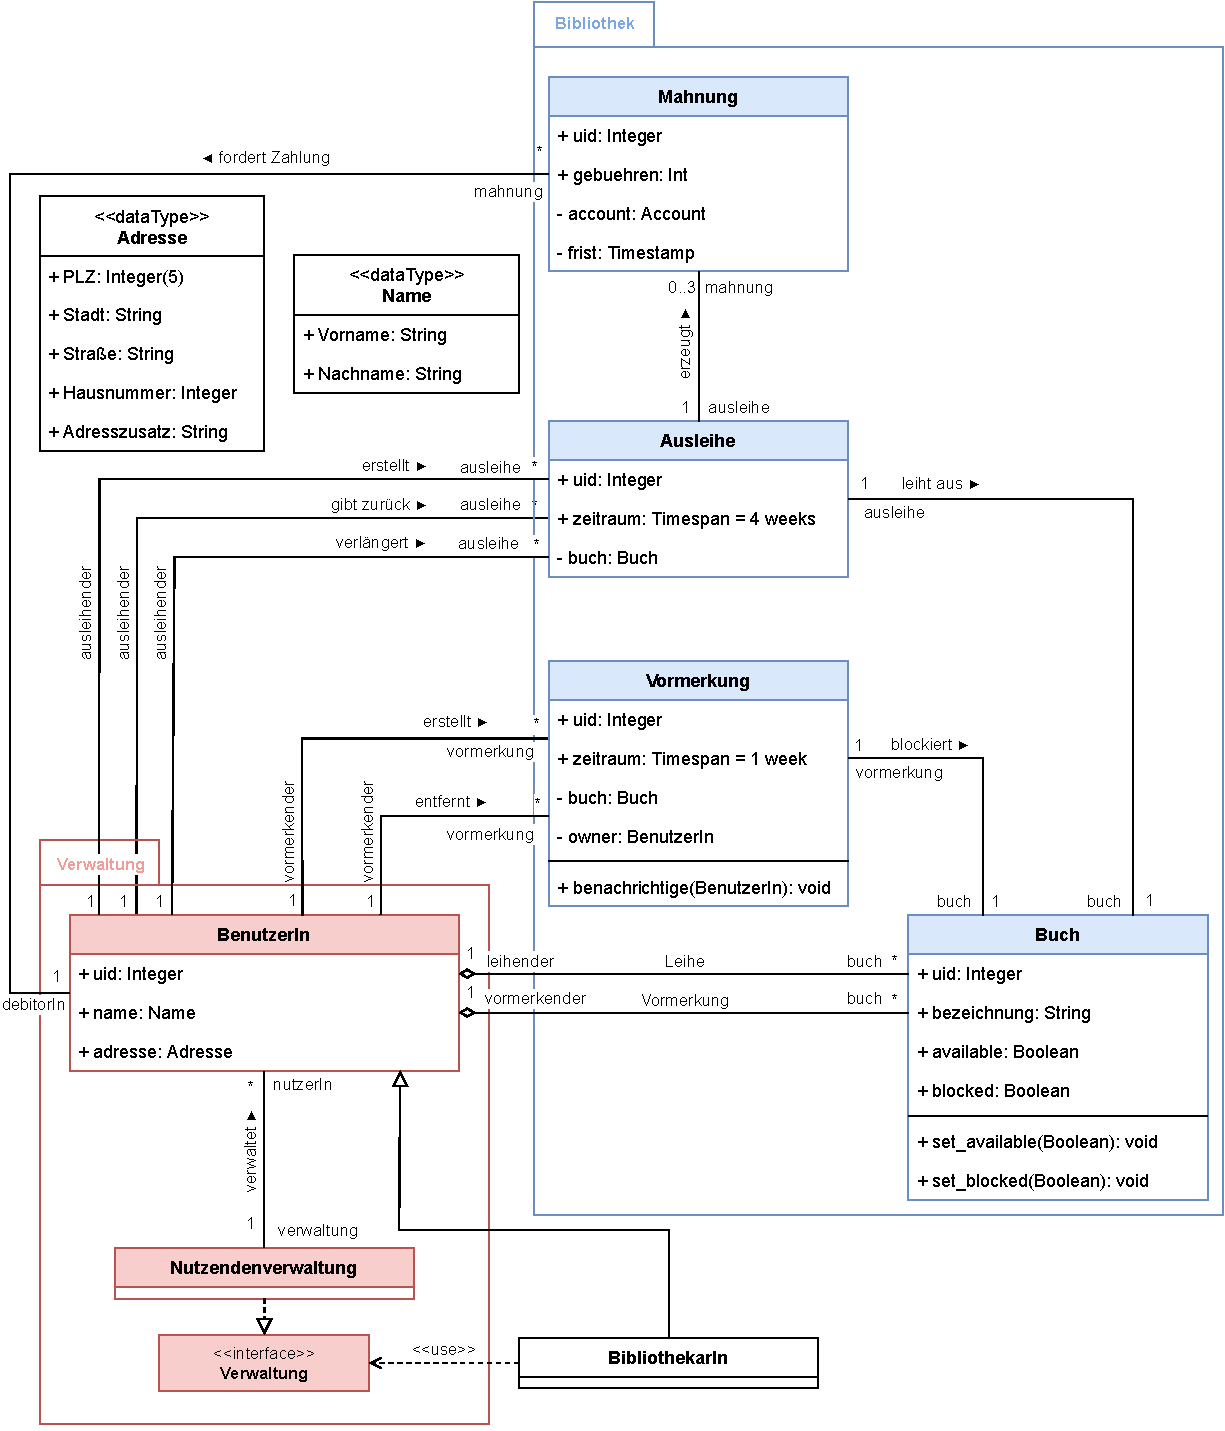
\includegraphics[width=\textwidth]{swt_h06_bibliothek.pdf}
        \end{center}
    \end{solution}
\end{questions}
\end{document}